\documentclass[../main.tex]{subfiles}
\usetikzlibrary{positioning, shapes.geometric, arrows.meta, fit,
decorations.pathreplacing}
\begin{document}

Chương 3 trình bày kiến trúc tổng thể và phương pháp nghiên cứu của
hệ thống Guepard
Shield. Nội dung chương mô tả chi tiết bốn giai đoạn của pipeline
đầu-cuối, bao gồm tiền
xử lý dữ liệu và token hóa tên lời gọi hệ thống (Giai đoạn 1), huấn
luyện mô hình
Transformer Teacher theo cơ chế dự đoán token tiếp theo (Giai đoạn
2), chưng cất tri
thức sang biểu diễn DFA Student thông qua gom cụm K-Means trên các
vector trạng thái ẩn
(Giai đoạn 3), và thực thi bảng chuyển trạng thái tại runtime bằng
eBPF (Giai đoạn 4).
Mỗi giai đoạn được trình bày cùng lý do thiết kế, các siêu tham số
kiểm soát và giao thức
đánh giá tương ứng.

\section{Tổng quan kiến trúc}
\label{sec:method_overview}

Guepard Shield được tổ chức thành một pipeline bốn giai đoạn như đã
mô tả tổng quát trong
Hình~\ref{fig:pipeline}. Ranh giới giữa hai giai đoạn đầu - học ngoại
tuyến (offline
learning) - và hai giai đoạn sau - thực thi trực tuyến (online
enforcement) - phản ánh
nguyên tắc thiết kế trung tâm của hệ thống: tách biệt giai đoạn học
biểu diễn phức tạp
ra khỏi giai đoạn kiểm tra nhẹ tại runtime.

\begin{figure}[!htbp]
  \centering
  \begin{tikzpicture}[
      node distance=1.2cm,
      block/.style={rectangle, draw, fill=blue!10, text width=9.5cm,
      align=center, rounded corners, minimum height=1cm, line width=0.8pt},
      line/.style={draw, -{Latex[scale=1.2]}, line width=1pt}
    ]
    \node [block] (input) {\textbf{Luồng Syscall Thô (Raw Syscall Stream)}};
    \node [block, below=of input] (phase1) {\textbf{Giai đoạn 1: Tiền
      xử lý dữ liệu}\\Tokenization tên syscall (Vocabulary) \& Tạo các
    sliding windows $W$};
    \node [block, below=of phase1] (phase2) {\textbf{Giai đoạn 2:
      Transformer Teacher (Mô hình huấn luyện)}\\Decoder-only, Causal
    Self-Attention, học hành vi bình thường};
    \node [block, below=of phase2] (phase3) {\textbf{Giai đoạn 3:
      Trích xuất DFA Student}\\Phân cụm K-Means các vector ẩn $h_t$ lớp
    cuối \& Cắt tỉa thống kê (S4)};
    \node [block, below=of phase3] (phase4) {\textbf{Giai đoạn 4:
      Thực thi eBPF Kernel}\\Nạp cấu hình dfa\_config.json vào BPF Maps
    \& Giám sát thời gian thực với độ phức tạp $O(1)$};

    \path [line] (input) -- (phase1);
    \path [line] (phase1) -- (phase2);
    \path [line] (phase2) -- (phase3);
    \path [line] (phase3) -- (phase4);
  \end{tikzpicture}
  \caption{Sơ đồ pipeline bốn giai đoạn của hệ thống Guepard Shield}
  \label{fig:pipeline}
\end{figure}

Ở giai đoạn ngoại tuyến, dữ liệu syscall bình thường được tiền xử lý
và token hóa (Giai
đoạn 1), sau đó được dùng để huấn luyện một mô hình Transformer
Decoder-only theo mục
tiêu next-token prediction (Giai đoạn 2). Khi mô hình Teacher hội tụ,
các vector trạng
thái ẩn lớp cuối của nó được trích xuất và rời rạc hóa thành một DFA
compact thông qua
gom cụm K-Means và xây dựng bảng chuyển trạng thái (Giai đoạn 3). Ở
giai đoạn trực
tuyến, bảng chuyển trạng thái DFA được nạp vào BPF Maps trong kernel;
chương trình eBPF
sau đó kiểm tra mỗi syscall với chi phí $O(1)$ trên mỗi sự kiện (Giai đoạn 4).

Cơ chế tương tác động giữa kernel space và user space được mô tả trong
Hình~\ref{fig:runtime}. Khi DFA phát hiện một bước chuyển trạng thái
trong vùng nghi vấn
(Suspect), sự kiện đó được chuyển lên Rust Agent ở user space thông
qua BPF perf ring buffer
để đánh giá sâu hơn bởi mô hình Transformer; nếu được xác định là
false positive, DFA
được cập nhật nguyên tử mà không cần tải lại kernel. Điều này cho
phép hệ thống tự điều
chỉnh trước các concept drift mà không gián đoạn giám sát thời gian thực.

\begin{figure}[!htbp]
  \centering
  \resizebox{\textwidth}{!}{
    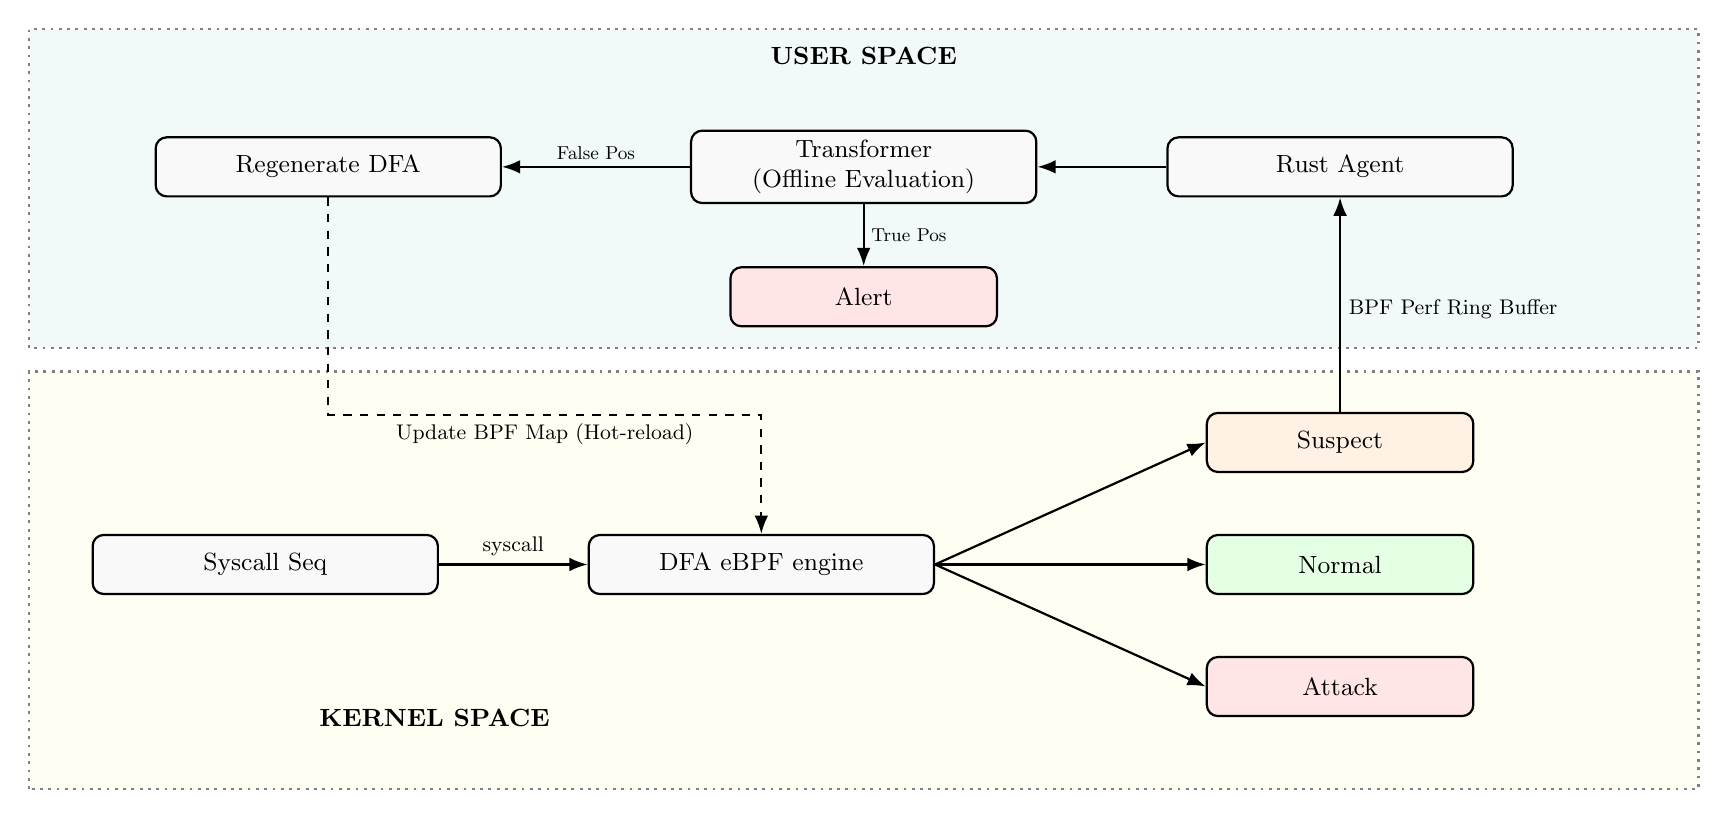
\begin{tikzpicture}[
        font=\small,
        block/.style={rectangle, draw, fill=gray!5, text
          width=4.15cm, align=center, rounded corners, minimum
        height=0.75cm, line width=0.8pt},
        action/.style={rectangle, draw, fill=red!10, text
          width=3.15cm, align=center, rounded corners, minimum
        height=0.75cm, line width=0.8pt},
        normal/.style={rectangle, draw, fill=green!10, text
          width=3.15cm, align=center, rounded corners, minimum
        height=0.75cm, line width=0.8pt},
        suspect/.style={rectangle, draw, fill=orange!10, text
          width=3.15cm, align=center, rounded corners, minimum
        height=0.75cm, line width=0.8pt},
        line/.style={draw, -{Latex[scale=1.0]}, line width=0.8pt},
        dashedline/.style={draw, dashed, -{Latex[scale=1.0]}, line width=0.8pt}
      ]
      \draw[fill=teal!5, draw=gray, dotted, line width=1pt] (-8.0,
      -2.15) rectangle (13.2, 1.9);
      \node at (2.6, 1.56) {\textbf{USER SPACE}};

      \draw[fill=yellow!5, draw=gray, dotted, line width=1pt] (-8.0,
      -7.75) rectangle (13.2, -2.45);
      \node[fill=yellow!5, inner sep=1pt] at (-2.85, -6.85)
      {\textbf{KERNEL SPACE}};

      \node [block] (u_agent) at (8.65, 0.15) {Rust Agent};
      \node [block] (u_teacher) at (2.6, 0.15) {Transformer
      \\(Offline Evaluation)};
      \node [block] (u_rebuild) at (-4.2, 0.15) {Regenerate DFA};
      \node [action] (u_alert) at (2.6, -1.5) {Alert};

      \node [block] (k_input) at (-5.0, -4.9) {Syscall Seq};
      \node [block] (k_dfa) at (1.3, -4.9) {DFA eBPF
      engine};

      \node [suspect] (k_suspect) at (8.65, -3.35) {Suspect};
      \node [normal] (k_norm) at (8.65, -4.9) {Normal};
      \node [action] (k_attack) at (8.65, -6.45) {Attack};

      \path [line] (k_input) -- node[above, scale=0.85] {syscall} (k_dfa);
      \path [line] (k_dfa.east) -- (k_norm.west);
      \path [line] (k_dfa.east) -- (k_attack.west);
      \path [line] (k_dfa.east) -- (k_suspect.west);

      \path [line] (k_suspect.north)
      -- node[right, scale=0.85] {BPF Perf Ring Buffer} (8.65, -0.35)
      -- (u_agent.south);

      \path [line] (u_agent) -- (u_teacher);
      \path [line] (u_teacher) -- node[right, scale=0.75] {True Pos} (u_alert);
      \path [line] (u_teacher) -- node[above, scale=0.75] {False Pos}
      (u_rebuild);

      \path [dashedline] (u_rebuild.south)
      -- (-4.2, -3.0)
      -- node[below, scale=0.85] {Update
      BPF Map (Hot-reload)} (1.3, -3.0)
      -- (k_dfa.north);

    \end{tikzpicture}
  }
  \caption{Cơ chế tương tác động và vòng lặp cập nhật giữa
  Kernel-space và User-space}
  \label{fig:runtime}
\end{figure}

Một điểm thiết kế quan trọng là hệ thống không ghi lại (record) toàn
bộ chuỗi syscall
tại runtime. Thay vào đó, chỉ tồn tại các cửa sổ trượt (sliding
windows) có kích thước
$W$ được duy trì liên tục theo từng định danh luồng (TID). Mỗi
syscall mới đẩy cửa sổ
tiến một bước, và DFA cập nhật trạng thái hiện tại dựa trên token tương ứng.

\section{Giai đoạn 1 - Tiền xử lý dữ liệu}
\label{sec:phase1}

Giai đoạn này chuyển đổi các bản ghi syscall thô từ bộ dữ liệu LID-DS-2021
\cite{grimmer2022dataset} thành các chuỗi token số nguyên và nhãn
phân loại phục vụ
cho các giai đoạn tiếp theo.

\subsection{Token hóa tên lời gọi hệ thống}
\label{sec:tokenization}

Mỗi sự kiện syscall được ánh xạ từ tên lời gọi hệ thống sang một chỉ
số nguyên thông
qua một bộ từ vựng cố định được xây dựng từ tập huấn luyện:

\begin{equation}
  \label{eq:tokenization}
  \text{token\_id}(s) = \text{vocab}[\text{Syscall\_Name}(s)]
\end{equation}

Bộ từ vựng được xây dựng với ngưỡng tần suất tối thiểu
$f_{\text{min}}$ để loại bỏ các syscall xuất hiện
quá thưa thớt trong dữ liệu huấn luyện \cite{mvula2023evaluating}.
Các tên syscall không
được nhận diện tại thời điểm inference được ánh xạ tới token đặc biệt
\texttt{<UNK>}.
Trong nghiên cứu này, cấu hình bộ từ vựng tham chiếu đạt kích thước
$|\Sigma| = 102$ trong thực nghiệm, bao phủ hầu hết các lời
gọi hệ thống xuất hiện trong các khối lượng công việc máy chủ bình thường.

Lý do chọn cách token hóa thuần túy dựa trên tên syscall là vì tên
syscall tạo thành một
bảng chữ cái hữu hạn và ổn định, thỏa mãn trực tiếp yêu cầu của DFA
về một bảng chữ cái
đầu vào hữu hạn $\Sigma$ mà không cần kỹ thuật mã hóa phức tạp. Đây
cũng là điều kiện
tiên quyết để chương trình eBPF có thể thực hiện ánh xạ từ tên
syscall sang token ID bằng
một thao tác tra cứu BPF Map đơn giản tại runtime.

Một hướng phát triển được dự kiến là token hóa tổng hợp (composite
tokenization), trong
đó mỗi syscall được ánh xạ sang một token hỗn hợp kết hợp tên và nhóm
mã trả về, ví dụ
\texttt{(Syscall\_Name, ReturnCode\_Bucket)}. Phương án này cho phép
phân biệt một lệnh
\texttt{open} thành công với một lệnh thất bại trả về EPERM, tăng
tính phong phú ngữ
nghĩa của bảng chữ cái. Tuy nhiên, mở rộng này làm tăng kích thước bộ
từ vựng và kích
thước BPF Map tương ứng, nên được hoãn lại sau khi hệ thống cơ sở được xác nhận.

Bảng~\ref{tab:vocab} trình bày một phần bộ từ vựng thực nghiệm, minh
họa cấu trúc
tuyến tính đơn giản của bảng tra cứu này. Toàn bộ ánh xạ được xây
dựng một lần duy
nhất trên tập huấn luyện và giữ cố định trong suốt vòng đời của mô
hình, đảm bảo sự
nhất quán giữa giai đoạn ngoại tuyến và giai đoạn thực thi eBPF.

\begin{table}[htbp]
  \caption{Ví dụ bộ từ vựng syscall: ánh xạ từ tên lời gọi hệ thống
    sang chỉ số token
    nguyên. Phần lớn token ID tương ứng với các syscall xuất hiện
    thường xuyên trong
  khối lượng công việc máy chủ; token 0 dành riêng cho \texttt{<UNK>}.}
  \label{tab:vocab}
  \centering
  \begin{tabular}{|l|c||l|c|}
    \hline
    \textbf{Tên syscall} & \textbf{Token ID} &
    \textbf{Tên syscall} & \textbf{Token ID} \\ \hline
    \texttt{<UNK>}    & 0  & \texttt{brk}       & 11 \\ \hline
    \texttt{read}     & 1  & \texttt{ioctl}     & 12 \\ \hline
    \texttt{write}    & 2  & \texttt{socket}    & 13 \\ \hline
    \texttt{open}     & 3  & \texttt{connect}   & 14 \\ \hline
    \texttt{close}    & 4  & \texttt{sendto}    & 15 \\ \hline
    \texttt{stat}     & 5  & \texttt{recvfrom}  & 16 \\ \hline
    \texttt{fstat}    & 6  & \texttt{execve}    & 17 \\ \hline
    \texttt{mmap}     & 7  & \texttt{clone}     & 18 \\ \hline
    \texttt{munmap}   & 8  & \texttt{futex}     & 19 \\ \hline
    \texttt{mprotect} & 9  & \texttt{poll}      & 20 \\ \hline
    \texttt{access}   & 10 & $\cdots$           & $\cdots$ \\ \hline
  \end{tabular}
\end{table}

\subsection{Phân đoạn cửa sổ trượt và gán nhãn}
\label{sec:windowing}

Chuỗi syscall theo từng luồng tiến trình được phân đoạn thành các cửa
sổ trượt gối đầu
có kích thước $W$ và bước nhảy $S$ \cite{grimmer2022improving}:

\begin{equation}
  \label{eq:window}
  w_i = [s_{iS+1},\ s_{iS+2},\ \ldots,\ s_{iS+W}]
\end{equation}

trong đó $W$ và $S$ là các siêu tham số đại diện cho kích thước cửa
sổ và bước nhảy (cấu hình tham chiếu trong thực nghiệm tương ứng là
$W = 64$, $S = 32$). Cửa sổ
kích thước nhỏ được lựa chọn vì ba lý do chính:

\begin{enumerate}
  \item \textbf{Tính cục bộ tạm thời của hành vi tấn công:} Phần lõi
    của một sự kiện
    khai thác thường hoàn thành trong vài chục syscall, nên một cửa
    sổ nhỏ đủ để bao
    phủ tín hiệu bất thường mà không cần ngữ cảnh quá dài.
  \item \textbf{Tính tổng quát hóa của mô hình Teacher:} Window nhỏ
    hơn buộc mô hình
    Transformer phải học biểu diễn tổng quát hơn thay vì ghi nhớ các
    chuỗi đặc trưng
    cụ thể, dẫn đến các vector trạng thái ẩn có phân cụm sạch hơn ở Giai đoạn 3.
  \item \textbf{Tính gọn nhẹ của DFA:} Số trạng thái DFA cần thiết phụ thuộc vào
    kích thước không gian trạng thái ẩn; window nhỏ hơn làm giảm sự
    đa dạng cần mô
    hình hóa, giúp DFA chiếm ít bộ nhớ kernel hơn.
\end{enumerate}

Hình~\ref{fig:windowing} minh họa quá trình phân đoạn với một chuỗi ví dụ.

\begin{figure}[H]
  \centering
  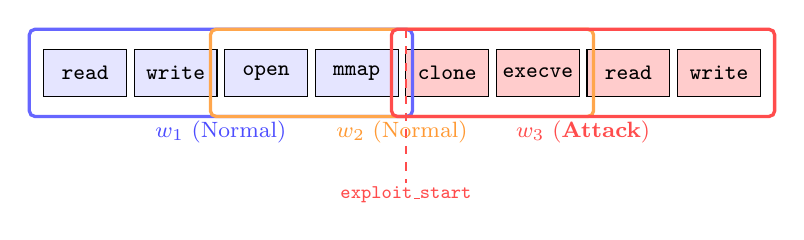
\begin{tikzpicture}[
      node distance=0.3cm and 0.0cm,
      tok/.style={rectangle, draw, fill=blue!10, minimum width=1.05cm,
      minimum height=0.6cm, font=\footnotesize, inner sep=2pt},
      atk/.style={rectangle, draw, fill=red!20, minimum width=1.05cm,
      minimum height=0.6cm, font=\footnotesize, inner sep=2pt}
    ]
    % Token row
    \node[tok] (t1) at (0,    0) {\texttt{read}};
    \node[tok] (t2) at (1.15, 0) {\texttt{write}};
    \node[tok] (t3) at (2.30, 0) {\texttt{open}};
    \node[tok] (t4) at (3.45, 0) {\texttt{mmap}};
    \node[atk] (t5) at (4.60, 0) {\texttt{clone}};
    \node[atk] (t6) at (5.75, 0) {\texttt{execve}};
    \node[atk] (t7) at (6.90, 0) {\texttt{read}};
    \node[atk] (t8) at (8.05, 0) {\texttt{write}};

    % exploit_start marker
    \draw[dashed, red!70, line width=0.9pt] (4.075, 0.55) -- (4.075, -1.4);
    \node[font=\scriptsize, red!70] at (4.075, -1.55) {\texttt{exploit\_start}};

    % Window 1
    \draw[draw=blue!60, line width=1.2pt, rounded corners=2pt]
    ([xshift=-5pt, yshift=-7pt]t1.south west)
    rectangle ([xshift=5pt, yshift=7pt]t4.north east);
    \node[font=\footnotesize, blue!70] at (1.725, -0.75) {$w_1$ (Normal)};

    % Window 2
    \draw[draw=orange!70, line width=1.2pt, rounded corners=2pt]
    ([xshift=-5pt, yshift=-7pt]t3.south west)
    rectangle ([xshift=5pt, yshift=7pt]t6.north east);
    \node[font=\footnotesize, orange!80] at (4.025, -0.75) {$w_2$ (Normal)};

    % Window 3
    \draw[draw=red!70, line width=1.2pt, rounded corners=2pt]
    ([xshift=-5pt, yshift=-7pt]t5.south west)
    rectangle ([xshift=5pt, yshift=7pt]t8.north east);
    \node[font=\footnotesize, red!70] at (6.325, -0.75) {$w_3$
    (\textbf{Attack})};

  \end{tikzpicture}
  \caption{Minh họa phân đoạn cửa sổ trượt với $W=4$, $S=2$. Các ô
    nền đỏ là các syscall
    xảy ra sau thời điểm \texttt{exploit\_start}. Window $w_3$ nhận
    nhãn Attack vì
    timestamp của syscall cuối cùng của nó nằm sau mốc khai thác;
    $w_1$ và $w_2$ nhận nhãn
  Normal dù có gối đầu với vùng attack.}
  \label{fig:windowing}
\end{figure}

Các window được gán nhãn bằng cách sử dụng dấu thời gian khai thác từ
tệp metadata JSON
của LID-DS: một window được gán nhãn \textbf{attack} nếu dấu thời
gian của syscall cuối
cùng trong window nằm trong khoảng thời gian khai thác của bản ghi
tương ứng; ngược lại
là \textbf{normal}. Nhãn này chỉ được sử dụng cho đánh giá ngoại
tuyến - không tham gia
vào quá trình huấn luyện mô hình, phù hợp với bài toán phát hiện bất
thường không giám
sát.

Cần lưu ý rằng bộ dữ liệu LID-DS gán nhãn attack cho toàn bộ phần
đuôi của bản ghi kể
từ thời điểm \texttt{exploit\_start} mà không xác định thời điểm kết
thúc khai thác. Hệ
quả thực nghiệm của đặc điểm gán nhãn này đối với việc diễn giải các
số liệu đánh giá
sẽ được phân tích định lượng và trình bày chi tiết trong Chương 5.

\section{Giai đoạn 2 - Huấn luyện Transformer Teacher}
\label{sec:phase2}

\subsection{Kiến trúc mô hình}
\label{sec:teacher_arch}

Mô hình Teacher được xây dựng dựa trên kiến trúc Transformer
Decoder-only với causal
self-attention như đã trình bày trong §\ref{sec:transformer}, áp dụng
trực tiếp cho chuỗi
token syscall \cite{fournier2023language,alsiam2026transcall}. Mặt nạ
nhân quả đảm bảo
tại mỗi vị trí $t$, vector trạng thái ẩn lớp cuối $h_t^{(L)}$ chỉ
được tính từ ngữ
cảnh $(s_1, \ldots, s_t)$. Điều này phản chiếu
đúng tính nhân quả của luồng syscall tại runtime: hệ thống không bao
giờ có thể biết
trước syscall tương lai.

Kiến trúc mô hình được tham số hóa bởi kích thước embedding $d$, số
lớp Transformer $L$, số attention heads $h$, kích thước feed-forward
$d_{\text{ff}}$, kích thước bộ từ vựng $|\Sigma|$ và kích thước cửa
sổ $W$. Trong nghiên cứu này, cấu hình tham chiếu trong thực nghiệm
gồm: $d = 128$, $L = 4$, $h = 4$, $d_{\text{ff}} = 512$, $|\Sigma| =
102$, và $W = 64$. Các lớp
chuẩn hóa sử dụng RMSNorm theo kiểu pre-norm, hàm kích hoạt GELU, và
mã hóa vị trí
xoay (Rotary Position Embedding - RoPE). Trọng số lớp nhúng đầu vào
và lớp chiếu đầu ra
được ràng buộc chung (weight tying) để giảm số tham số và cải thiện
tổng quát hóa. Hình~\ref{fig:transformer_arch} mô tả sơ đồ kiến trúc đầy đủ.

Lựa chọn Decoder-only thay vì một kiến trúc encoder kiểu BERT xuất
phát từ bản chất
thời gian của bài toán syscall. Trong mô hình encoder hai chiều, mỗi
vị trí có thể
chú ý đồng thời tới các token đứng trước và đứng sau nó; cách này hữu
ích cho các bài
toán hiểu câu ngoại tuyến, nhưng không phản ánh đúng điều kiện vận
hành của một bộ
giám sát runtime, nơi quyết định tại thời điểm $t$ chỉ được phép dựa
trên lịch sử đã
xảy ra. Nếu sử dụng encoder để tạo biểu diễn cho token giữa cửa sổ,
vector ẩn đó có
thể đã chứa thông tin từ các syscall tương lai trong cùng window, tạo
ra một dạng rò
rỉ ngữ cảnh (future leakage). Điều này làm điểm đánh giá ngoại tuyến
có thể trở nên
lạc quan hơn thực tế và, quan trọng hơn, phá vỡ giả định dùng $h_t$
như một trạng thái
nhân quả khi trích xuất bảng chuyển DFA ở Giai đoạn 3. Mô hình
Decoder-only với causal
mask tránh vấn đề này: vector $h_t$ là biểu diễn của đúng tiền tố
$(s_1,\ldots,s_t)$,
tương tự một trạng thái tóm tắt lịch sử đã quan sát của luồng syscall.

Một kiến trúc encoder như BERT cũng thường được huấn luyện bằng
masked-token modeling
hoặc dùng vector tổng hợp cấp chuỗi như \texttt{[CLS]} cho phân loại
\cite{devlin2019bert}.
Hai cơ chế này không khớp trực tiếp với mục tiêu của Guepard Shield.
Hệ thống cần một
tín hiệu dự đoán tuần tự $P(s_{t+1}\mid s_1,\ldots,s_t)$ để vừa chấm
điểm bất thường
bằng NLL, vừa tạo cặp chuyển tiếp $(h_t, s_{t+1}, h_{t+1})$ phục vụ
chưng cất automata.
Nếu mô hình chỉ tạo một embedding cấp window, việc ánh xạ embedding
đó thành các trạng
thái trung gian của DFA sẽ kém tự nhiên hơn, vì DFA cần cập nhật
trạng thái sau mỗi
syscall chứ không chỉ đưa ra một nhãn cho toàn bộ cửa sổ. Do đó,
Decoder-only được chọn
không phải vì encoder yếu hơn về mặt biểu diễn, mà vì nó bảo toàn cấu
trúc nhân quả và
cấu trúc chuyển trạng thái mà pipeline DFA yêu cầu.

Cơ chế self-attention được dùng vì hành vi hệ thống không chỉ phụ
thuộc vào syscall
ngay trước đó. Một lời gọi như \texttt{open}, \texttt{read} hoặc
\texttt{mmap} có thể
mang ý nghĩa khác nhau tùy vào chuỗi ngữ cảnh trước đó: tiến trình
đang khởi tạo, đang
xử lý kết nối, đang nạp thư viện, hay đang thực hiện một chuỗi thao
tác hiếm gặp. Các
mô hình Markov bậc thấp hoặc n-gram chỉ nhìn được một vùng ngữ cảnh
cố định ngắn; trong
khi đó, multi-head self-attention cho phép mỗi vị trí kết hợp thông
tin từ nhiều điểm
trước đó trong window. Nhiều attention head cũng giúp mô hình học các
kiểu quan hệ
khác nhau giữa syscall: một head có thể tập trung vào các mẫu I/O lặp
lại, một head
khác vào chuỗi tạo tiến trình hoặc ánh xạ bộ nhớ. Trong nghiên cứu
này số head được
giữ ở mức $h=4$ để cân bằng giữa năng lực biểu diễn và chi phí trích
xuất trạng thái
ẩn ngoại tuyến.

Vì self-attention tự thân không biết thứ tự của token, mô hình cần
một cơ chế mã hóa
vị trí. Thứ tự là thông tin cốt lõi trong syscall IDS: hai cửa sổ có
cùng tập syscall
nhưng thứ tự khác nhau có thể biểu diễn hai hành vi hoàn toàn khác
nhau. RoPE được chọn
vì nó đưa thông tin vị trí vào phép tính attention theo dạng tương
đối giữa Query và
Key, thay vì chỉ cộng một vector vị trí tuyệt đối vào embedding đầu
vào \cite{su2024roformer}.
Điều này phù hợp với dữ liệu cửa sổ trượt, nơi cùng một mẫu hành vi
có thể xuất hiện
ở các vị trí hơi khác nhau trong window. Với RoPE, mô hình vẫn biết
khoảng cách và thứ
tự tương đối giữa các syscall, trong khi ít phụ thuộc hơn vào việc
một syscall cụ thể
nằm đúng ở vị trí tuyệt đối nào. Đây là một đặc tính hữu ích khi mục
tiêu cuối không
chỉ là dự đoán token, mà còn là tạo ra các hidden state đủ ổn định để
gom cụm bằng
K-Means.

Mỗi block Transformer được tổ chức theo dạng pre-norm, đặt RMSNorm
trước self-attention
và trước FFN. Thiết kế pre-norm giúp đường truyền gradient ổn định
hơn khi xếp chồng
nhiều lớp, vì nhánh residual luôn cung cấp một đường đi gần tuyến
tính từ đầu vào tới
đầu ra của block. RMSNorm được dùng thay cho LayerNorm đầy đủ vì nó
chuẩn hóa theo độ
lớn căn trung bình bình phương của vector, bỏ qua bước trừ trung
bình, nhờ đó đơn giản
hơn về mặt tính toán nhưng vẫn kiểm soát được thang đo activation
\cite{zhang2019rmsnorm}.
Trong bối cảnh mô hình Teacher chỉ cần đủ mạnh để học manifold hành
vi bình thường và
trích xuất embedding ổn định, RMSNorm là một lựa chọn thực dụng: giảm
độ phức tạp nhỏ
nhưng giữ được lợi ích ổn định huấn luyện của normalization.

Residual connection xuất hiện sau cả lớp attention và lớp FFN vì mỗi
sub-layer chỉ nên
học phần hiệu chỉnh so với biểu diễn hiện tại, không phải học lại
toàn bộ thông tin
lịch sử từ đầu \cite{he2016resnet}. Đối với chuỗi syscall, điều này
đặc biệt quan
trọng: nhiều token trong window thuộc các mẫu bình thường lặp lại,
nên biểu diễn ngữ
cảnh đã tích lũy ở lớp trước cần được bảo toàn trong khi attention
hoặc FFN bổ sung các
quan hệ mới. Nếu bỏ residual connection, các lớp sâu hơn dễ làm mất
hoặc bóp méo tín
hiệu ngữ cảnh ban đầu, khiến hidden state cuối biến động mạnh hơn và
khó gom cụm thành
các trạng thái DFA ổn định. Nói cách khác, residual connection không
chỉ giúp tối ưu hóa
mô hình nơ-ron, mà còn gián tiếp làm bước rời rạc hóa ở Giai đoạn 3
dễ kiểm soát hơn.

Khối FFN gồm hai phép chiếu tuyến tính với GELU ở giữa đóng vai trò
biến đổi phi tuyến
theo từng vị trí token. Self-attention trộn thông tin giữa các vị trí
trong window,
trong khi FFN xử lý lại biểu diễn tại từng vị trí để tạo các đặc
trưng bậc cao hơn.
Kích thước ẩn $d_{\text{ff}}=512$ lớn hơn kích thước embedding
$d=128$ nhằm tạo không
gian trung gian đủ rộng cho các tương tác phi tuyến, sau đó nén trở
lại không gian
trạng thái ẩn dùng chung. GELU được chọn vì là hàm kích hoạt trơn,
thường được dùng
trong Transformer hiện đại, giúp mô hình biểu diễn các biến đổi mềm
thay vì ngưỡng hóa
cứng như ReLU \cite{hendrycks2016gelu}. Cuối cùng, weight tying giữa
embedding đầu vào
và projection đầu ra tận dụng cùng một không gian biểu diễn cho token
syscall khi đọc
vào và khi dự đoán ra \cite{press2017using}. Với bảng chữ cái syscall
tương đối nhỏ,
ràng buộc này giảm số tham số không cần thiết và khuyến khích biểu
diễn token nhất quán
hơn giữa hai đầu của mô hình.

\begin{figure}[H]
  \centering
  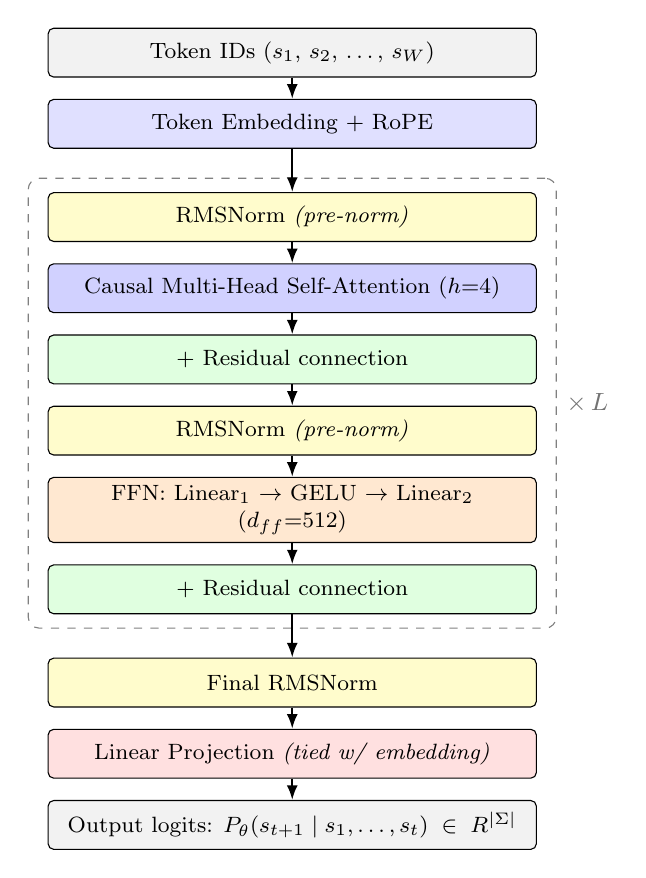
\begin{tikzpicture}[
      node distance=0.27cm,
      blk/.style={rectangle, draw, minimum width=6.2cm, minimum height=0.62cm,
      align=center, font=\footnotesize, rounded corners=2pt, inner sep=3pt},
      arr/.style={draw, -{Latex[scale=0.8]}, line width=0.8pt}
    ]
    \node[blk, fill=gray!10] (input)
    {Token IDs $(s_1,\, s_2,\, \ldots,\, s_W)$};
    \node[blk, fill=blue!12, below=of input] (emb)
    {Token Embedding $+$ RoPE};
    % === Transformer block (repeated L times) ===
    \node[blk, fill=yellow!20, below=0.55cm of emb] (rn1)
    {RMSNorm \emph{(pre-norm)}};
    \node[blk, fill=blue!18, below=of rn1] (mha)
    {Causal Multi-Head Self-Attention ($h{=}4$)};
    \node[blk, fill=green!12, below=of mha] (res1)
    {$+$ Residual connection};
    \node[blk, fill=yellow!20, below=of res1] (rn2)
    {RMSNorm \emph{(pre-norm)}};
    \node[blk, fill=orange!18, below=of rn2, text width=5.8cm] (ffn)
    {FFN: Linear$_1$ $\to$ GELU $\to$ Linear$_2$\\($d_\text{ff}{=}512$)};
    \node[blk, fill=green!12, below=of ffn] (res2)
    {$+$ Residual connection};
    % Dashed box around L-repeated block
    \node[draw=black!50, dashed, rounded corners=4pt,
      fit=(rn1)(res2), inner xsep=7pt, inner ysep=5pt,
    label={[font=\small, text=black!55]right:$\times\, L$}] {};
    % === End transformer block ===
    \node[blk, fill=yellow!20, below=0.55cm of res2] (fnorm)
    {Final RMSNorm};
    \node[blk, fill=red!12, below=of fnorm] (proj)
    {Linear Projection \emph{(tied w/ embedding)}};
    \node[blk, fill=gray!10, below=of proj] (output)
    {Output logits: $P_\theta(s_{t+1} \mid s_1, \ldots,
    s_t)\;\in\;\mathbb{R}^{|\Sigma|}$};
    % Arrows
    \draw[arr] (input) -- (emb);
    \draw[arr] (emb)   -- (rn1);
    \draw[arr] (rn1)   -- (mha);
    \draw[arr] (mha)   -- (res1);
    \draw[arr] (res1)  -- (rn2);
    \draw[arr] (rn2)   -- (ffn);
    \draw[arr] (ffn)   -- (res2);
    \draw[arr] (res2)  -- (fnorm);
    \draw[arr] (fnorm) -- (proj);
    \draw[arr] (proj)  -- (output);
  \end{tikzpicture}
  \caption{Kiến trúc Transformer Decoder-only của mô hình Teacher với
    $L{=}4$ lớp
    ($d{=}128$, $h{=}4$, $d_\text{ff}{=}512$). Cấu trúc Pre-Norm đặt RMSNorm
    \emph{trước} mỗi sub-layer, cải thiện ổn định gradient trong huấn luyện sâu.
    Mặt nạ nhân quả (causal mask) trong MHA đảm bảo $h_t$ chỉ phụ thuộc ngữ cảnh
    $(s_1, \ldots, s_t)$, phản ánh đúng tính nhân quả của luồng
    syscall tại runtime.
    Trọng số embedding và projection được ràng buộc chung (weight
    tying) để giảm số
  tham số.}
  \label{fig:transformer_arch}
\end{figure}

Mô hình được huấn luyện \textbf{chỉ trên các window bình thường} theo
tiêu chí dự đoán
token tiếp theo (next-token prediction) với hàm mất mát cross-entropy, theo công
thức~(\ref{eq:loss}) đã định nghĩa ở §\ref{sec:transformer}. Đây là
phương pháp phát
hiện bất thường không giám sát (unsupervised anomaly detection) \cite{pang2021deep} đã
được áp dụng rộng rãi
trong các hệ thống HIDS dựa trên chuỗi sự kiện
\cite{du2017deeplog,fournier2023language}:
mô hình học phân phối xác suất $P(\text{hành vi bình thường})$; các
window bất thường
biểu hiện dưới dạng xác suất thấp tương ứng với điểm Negative
Log-Likelihood cao tại
thời điểm inference.

Quá trình tối ưu hóa sử dụng AdamW \cite{loshchilov2019adamw} với lịch trình suy giảm học suất
cosine \cite{loshchilov2017sgdr} và giai đoạn
khởi động (warmup) chiếm 5\% tổng số bước huấn luyện. Kỹ thuật
Teacher Forcing \cite{williams1989teacher} cho phép
song song hóa quá trình huấn luyện trên toàn bộ chuỗi trong một
forward pass. Độ chính
xác hỗn hợp (AMP 16-bit mixed precision) \cite{micikevicius2018mixed} được áp dụng để giảm thời
gian huấn luyện và
bộ nhớ GPU cần thiết.

\subsection{Điểm bất thường dựa trên NLL của token cuối}
\label{sec:anomaly_score}

Đối với một window $w = [s_1, \ldots, s_W]$, điểm bất thường được
định nghĩa là giá trị
Negative Log-Likelihood (NLL) của \textbf{token cuối cùng} $s_W$ khi
đặt trong ngữ cảnh
$W-1$ token đứng trước:

\begin{equation}
  \label{eq:anomaly_score}
  \text{score}(w) = -\log P_\theta(s_W \mid s_1, \ldots, s_{W-1})
\end{equation}

Thiết kế chỉ tính điểm trên token cuối cùng phù hợp với quy tắc gán
nhãn window của
LID-DS: một window bị gán nhãn attack khi dấu thời gian của syscall
cuối cùng của nó nằm
trong khoảng khai thác, do đó điểm bất thường nhắm vào cùng vị trí.
Cách tính này đồng
thời tạo ra một ánh xạ tự nhiên sang Giai đoạn 3: vector $h_{W-1}$ -
trạng thái ẩn được
sử dụng để dự đoán $s_W$ - tích lũy toàn bộ lịch sử ngữ cảnh của
window và là ứng viên
trực tiếp để rời rạc hóa thành trạng thái DFA.

Cách tính điểm bất thường dựa trên NLL của token cuối cũng được so sánh với hai
phương án thay thế trong giai đoạn thiết kế:

\begin{itemize}
  \item \textbf{NLL trung bình toàn window:}
    \[
      \overline{\text{NLL}}(w) = -\frac{1}{W}\sum_{t=1}^{W}
      \log P_\theta(s_t \mid s_1, \ldots, s_{t-1})
    \]
    Cách tính này phân bổ đều tín hiệu bất thường trên toàn bộ chuỗi.
    Tuy nhiên, do
    các token đầu window thường thuộc vùng hành vi bình thường (xảy
      ra trước thời điểm
    khai thác), chúng đóng góp giá trị NLL thấp vào trung bình và pha
    loãng tín hiệu
    tấn công tập trung ở cuối window.
  \item \textbf{NLL tối đa trong window:}
    $\text{score}_{\max}(w) = \max_{1 \leq t \leq W}\bigl(-\log
      P_\theta(s_t \mid
    s_1, \ldots, s_{t-1})\bigr)$.
    Phương án này nhạy hơn với các sự kiện cục bộ bất thường, nhưng
    không nhất quán
    với quy tắc gán nhãn của LID-DS: token có NLL cao nhất không bảo
    đảm là token cuối
    cùng, dẫn đến sự không khớp giữa điểm số và nhãn window.
\end{itemize}

Một hạn chế quan trọng hơn của toàn bộ hướng tiếp cận ngưỡng NLL là
\textbf{tính bất
ổn định giữa các kịch bản}: giá trị ngưỡng tối ưu khác nhau đáng kể
giữa các kịch bản
tấn công khác nhau, thậm chí giữa các phiên làm việc trong cùng một
kịch bản. Điều
chỉnh ngưỡng thích ứng tại runtime trong môi trường nhân kernel là
không thực tế. Chính
hạn chế này là lý do kỹ thuật trực tiếp dẫn đến thiết kế DFA Student
ở Giai đoạn 3:
thay vì so sánh với một giá trị ngưỡng liên tục cần hiệu chuẩn lại,
quyết định phát
hiện được chuyển sang không gian trạng thái rời rạc trong đó nhãn attack đến từ
\textbf{bất thường cấu trúc} - bước chuyển trạng thái không tồn tại
trong bảng - thay
vì so sánh ngưỡng số.

Số liệu đánh giá chính của mô hình Teacher bao gồm AUROC và F1 ở cấp
độ cửa sổ so với
nhãn exploit-timestamp. AUROC và F1 ở cấp độ bản ghi
(recording-level) - thông qua
max-pooling điểm số trên từng bản ghi - được báo cáo như một chẩn
đoán bổ sung để phù
hợp với giao thức đánh giá LID-DS tiêu chuẩn \cite{grimmer2022dataset}.

\section{Giai đoạn 3 - Chưng cất DFA Student}
\label{sec:phase3}

Giai đoạn này chưng cất tri thức đã học của mô hình Transformer
Teacher thành một DFA
Student compact theo hướng trích xuất automata và chưng cất tri thức
từ mạng nơ-ron
\cite{ables2024eclectic,herbinger2023leveraging,friedman2023learning},
điều chỉnh cho
kiến trúc Transformer Decoder-only và bài toán chuỗi syscall. Quá
trình gồm bốn bước tuần tự: trích xuất
trạng thái ẩn, rời rạc hóa bằng K-Means, xây dựng bảng chuyển trạng
thái, và giải quyết
tính không xác định.

\subsection{Định nghĩa và trích xuất trạng thái ẩn}
\label{sec:hidden_states}

Trạng thái ẩn dùng để rời rạc hóa là vector nhúng đầu ra lớp
Transformer cuối cùng tại
vị trí token cuối của mỗi forward pass:

\begin{equation}
  \label{eq:hidden_state}
  h_t = \text{TransformerFinalLayer}(s_1, \ldots, s_t)[\text{vị trí } t]
  \in \mathbb{R}^d
\end{equation}

Nhờ cơ chế causal self-attention đã trình bày trong
§\ref{sec:transformer}, $h_t$ mã hóa
toàn bộ lịch sử nhân quả $(s_1, \ldots, s_t)$ trong một vector duy
nhất, đóng vai trò
tương tự trạng thái ẩn của RNN \cite{weiss2018extracting}. Đây là thành
phần tự nhiên nhất
để biểu diễn trạng thái DFA, vì một trạng thái DFA theo định nghĩa hình thức ở
§\ref{sec:dfa} cũng phải mã hóa toàn bộ thông tin từ lịch sử chuỗi
đầu vào cần thiết
cho các quyết định chuyển trạng thái tương lai.

Để đảm bảo tất cả các vector trạng thái ẩn được trích xuất đều có ngữ
cảnh đầy đủ $W$
token, các vector trạng thái ẩn được trích xuất từ tập dữ liệu huấn
luyện bình thường. Nhằm tối ưu hóa dung lượng lưu trữ trung gian và
chi phí tính toán ngoại tuyến, quá trình trích xuất này được thực
hiện với một bước nhảy thưa (stride $S_{\text{extract}} > 1$) thay vì
trích xuất dày đặc từng bước một. Tuy nhiên, tại thời điểm thực thi ở
nhân hệ điều hành, chương trình eBPF phải giám sát và duyệt trạng
thái DFA trên từng lời gọi hệ thống đơn lẻ (tương ứng với bước nhảy
$S = 1$). Sự không khớp về bước nhảy này (stride mismatch) tạo ra một
bài toán kỹ thuật: nếu xây dựng bảng chuyển trạng thái trực tiếp từ
các trạng thái ẩn thưa, bước chuyển trạng thái sẽ nhảy qua nhiều
syscall thay vì chuyển tiếp tuần tự trên từng syscall một.

Để giải quyết bài toán không khớp bước nhảy này mà không làm bùng nổ
không gian lưu trữ trung gian, hệ thống áp dụng cơ chế stream hai pha
(two-pass streaming) trên dữ liệu huấn luyện:
\begin{enumerate}
  \item \textbf{Pha 1 (Gom cụm thưa):} Tập huấn luyện được quét hai
    lần. Lần quét thứ nhất chỉ đếm số cửa sổ hợp lệ để xác định trước
    kích thước của ma trận trạng thái ẩn và bảng metadata. Lần quét
    thứ hai đưa từng batch cửa sổ qua bộ mã hóa của Transformer, lấy
    vector $h_t$ tại vị trí cuối cửa sổ và ghi tuần tự vào ma trận
    trạng thái ẩn. Metadata đi kèm mỗi vector gồm định danh bản ghi,
    vị trí bắt đầu của cửa sổ trong bản ghi, và token cuối của cửa
    sổ. Trong cấu hình tham chiếu, pha này sử dụng stride $4$ và lưu
    trạng thái ẩn ở độ chính xác thấp hơn để giảm dung lượng trung
    gian, trong khi các tham số hình dạng như số cửa sổ $M$, số chiều
    $d$, kích thước cửa sổ $W$, kích thước từ vựng và stride được lưu
    như metadata của thí nghiệm.
  \item \textbf{Pha 2 (Dựng bước chuyển dày):} Sau khi đã học được
    các tâm cụm, toàn bộ chuỗi syscall huấn luyện được stream lại với
    bước nhảy dày $S = 1$. Tại mỗi vị trí $t$, cửa sổ ngữ cảnh đầy đủ
    được đưa qua Transformer để tính vector trạng thái ẩn $h_t$, sau
    đó vector này được chiếu ngay vào tâm cụm gần nhất để xác định
    trạng thái DFA tương ứng. Các bước chuyển tiếp trạng thái tuần tự
    giữa hai thời điểm liên tiếp $(q_t, s_{t+1}) \to q_{t+1}$ được
    tích lũy trực tiếp vào bảng đếm. Nhờ cơ chế chiếu trực tiếp này,
    hệ thống không cần lưu toàn bộ hidden states stride-1 xuống đĩa,
    nhưng vẫn xây dựng được DFA đúng với từng syscall đơn lẻ.
\end{enumerate}
Cách tiếp cận này đảm bảo mỗi trạng thái DFA đại diện cho một ngữ
cảnh đầy đủ và ổn định, đồng thời bảo toàn tính chính xác của các
bước chuyển tiếp đơn bước trong nhân hệ điều hành. Các tham số cụ thể
như độ dài bước nhảy thưa $S_{\text{extract}}$ và các phân tích hiệu
năng liên quan sẽ được trình bày trong Chương 5. Thuật
toán~\ref{alg:extract_hidden_states_for_kmeans} mô tả cụ thể bước
trích xuất ma trận hidden states làm đầu vào cho K-Means: trước hết
đếm số cửa sổ hợp lệ để cấp phát bộ nhớ, sau đó đưa các cửa sổ qua
Transformer theo batch và ghi lại vector trạng thái ẩn tại token cuối
cùng cùng với metadata ánh xạ.

\begin{algorithm}[H]
  \caption{Trích xuất hidden states của Transformer làm đầu vào cho
  K-Means}
  \label{alg:extract_hidden_states_for_kmeans}
  \SetAlgoLined
  \DontPrintSemicolon
  \KwIn{Tập bản ghi huấn luyện bình thường $\mathcal{R}_{train}$;
    Transformer Teacher $F_\theta$; bộ từ vựng $\nu$; kích thước cửa
  sổ $W$; stride trích xuất $S_{\text{extract}}$; batch size $B$}
  \KwOut{Ma trận trạng thái ẩn $H \in \mathbb{R}^{M \times d}$ và
  bảng metadata $A \in \mathbb{Z}^{M \times 3}$}

  $M \gets 0$\;
  \ForEach{$r \in \mathcal{R}_{train}$}{
    $(x_1,\ldots,x_{|r|}) \gets \operatorname{tokenize}(r,\nu)$\;
    $M \gets M + \operatorname{count\_windows}(|r|, W,
    S_{\text{extract}})$\;
  }

  $H \gets \operatorname{zeros}(M,d)$;\quad
  $A \gets \operatorname{zeros}(M,3)$\;
  $m \gets 1$\;
  \ForEach{$r \in \mathcal{R}_{train}$}{
    $(x_1,\ldots,x_{|r|}) \gets \operatorname{tokenize}(r,\nu)$\;
    $\mathcal{W} \gets \operatorname{windows}(x, W,
    S_{\text{extract}})$\;
    \ForEach{$\mathcal{B} \in \operatorname{batches}(\mathcal{W},B)$}{
      $Z \gets \operatorname{last\_hidden}(F_\theta,\mathcal{B})$\;
      \ForEach{$(h,j) \in Z$}{
        $H[m] \gets h$\;
        $A[m] \gets (\mathrm{id}(r), j, x_{j+W-1})$\;
        $m \gets m + 1$\;
      }
    }
  }
  \Return{$(H,A)$}\;
\end{algorithm}

Lựa chọn vị trí token cuối cùng để lấy trạng thái ẩn cũng được so sánh với hai
chiến lược thay thế phổ biến:

\begin{itemize}
  \item \textbf{Mean pooling} $\bar{h} = \frac{1}{W}\sum_{t=1}^{W}
    h_t^{(L)}$: Phép
    trung bình hóa tất cả các vị trí trong window tạo ra một biểu diễn cấp câu
    (sentence-level), nhưng pha loãng thông tin ngữ cảnh đặc thù của
    thời điểm hiện
    tại. Với chuỗi syscall, các token giữa window mang biểu diễn của
    các trạng thái
    trung gian không nhất thiết liên quan đến quyết định tại thời
    điểm cuối; đưa chúng
    vào trung bình làm giảm tính phân biệt của các cụm K-Means.
  \item \textbf{Token [CLS] chuyên dụng}: Kiến trúc Encoder-only (BERT) sử dụng
    token [CLS] với bidirectional attention để tổng hợp biểu diễn cấp chuỗi. Tuy
    nhiên, mô hình Teacher sử dụng causal attention, trong đó không
    có vị trí nào
    có thể nhìn thấy toàn bộ chuỗi đầy đủ ngoại trừ token cuối cùng. Thêm token
    [CLS] với cơ chế đặc biệt sẽ đòi hỏi thay đổi kiến trúc và mục tiêu huấn
    luyện, phá vỡ tính nhất quán giữa giai đoạn huấn luyện và giai
    đoạn trích xuất.
\end{itemize}

Do đó, $h_{W-1}$ là lựa chọn tự nhiên, nhất quán với kiến trúc nhân quả, và hiệu
quả nhất về mặt tính toán: nó là vector duy nhất trong mỗi forward
pass đã tích lũy
toàn bộ lịch sử $W$ token, không cần bất kỳ bước xử lý bổ sung nào.

\subsection{Rời rạc hóa trạng thái bằng K-Means}
\label{sec:kmeans}

Tập hợp các vector $\{h_t\}_{t=1}^{N}$ thu được từ toàn bộ tập huấn
luyện được áp dụng
thuật toán gom cụm K-Means \cite{lloyd1982kmeans} với $K$ cụm. Mỗi tâm cụm $c_k$ định nghĩa
một trạng thái
DFA $q_k \in Q$; một vector $h$ được ánh xạ tới trạng thái $q_k$ trong đó:

\begin{equation}
  \label{eq:kmeans}
  \text{cluster}(h) = \arg\min_{k \in \{1,\ldots,K\}} \|h - c_k\|_2
\end{equation}

Về mặt thuật toán, hệ thống sử dụng biến thể mini-batch của K-Means \cite{sculley2010webscale}
thay vì K-Means toàn
phần, vì ma trận trạng thái ẩn có thể lớn hơn bộ nhớ RAM nếu nạp toàn
bộ ở độ chính xác
huấn luyện. Ở mỗi epoch, thuật toán đọc tuần tự các chunk trạng thái
ẩn, chuyển chúng về
độ chính xác tính toán phù hợp, rồi cập nhật tâm cụm bằng quy tắc
mini-batch. Sau khi
các tâm cụm hội tụ, toàn bộ ma trận trạng thái ẩn được quét lại để
gán nhãn cụm cho
từng cửa sổ; kết quả là một dãy nhãn trạng thái rời rạc có cùng thứ
tự với các cửa sổ
huấn luyện, còn các tâm cụm được giữ lại để chiếu các hidden state
mới trong pha dựng
bước chuyển dày. Các giá trị $K \in \{64,128,256,512\}$ được huấn
luyện độc lập để đánh
giá đánh đổi giữa độ mịn của rời rạc hóa và kích thước DFA. Vì vậy,
K-Means ở đây không
được hiểu là một bộ phân loại normal/attack trực tiếp; nó chỉ biến
không gian trạng thái
ẩn liên tục của Transformer thành các chỉ số trạng thái rời rạc mà
bảng chuyển DFA có
thể sử dụng.

Hình~\ref{fig:kmeans} minh họa quá trình ánh xạ từ không gian liên
tục $\mathbb{R}^d$
sang các trạng thái DFA rời rạc.

\begin{figure}[!htbp]
  \centering
  \begin{tikzpicture}[
      node distance=1.0cm and 1.4cm,
      hvec/.style={rectangle, draw, fill=blue!10, text width=1.8cm,
        align=center,
      minimum height=0.65cm, font=\footnotesize, rounded corners=2pt},
      state/.style={circle, draw, fill=orange!20, minimum size=0.85cm,
      font=\footnotesize, inner sep=1pt},
      kmbox/.style={rectangle, draw, fill=gray!10, text width=2.2cm,
        align=center,
      minimum height=3.6cm, rounded corners=4pt, font=\footnotesize},
      line/.style={draw, -{Latex[scale=0.9]}, line width=0.8pt}
    ]
    % Hidden state vectors
    \node[hvec] (h1) at (0,  0.6) {$h_{t_1} \in \mathbb{R}^{128}$};
    \node[hvec] (h2) at (0, -0.1) {$h_{t_2} \in \mathbb{R}^{128}$};
    \node[hvec] (h3) at (0, -0.8) {$h_{t_3} \in \mathbb{R}^{128}$};
    \node[hvec] (h4) at (0, -1.5) {$h_{t_4} \in \mathbb{R}^{128}$};
    \node[font=\scriptsize] at (0, -2.1) {$\vdots$};
    \node[font=\footnotesize\bfseries] at (0, 1.2) {Trạng thái ẩn};

    % K-Means box
    \node[kmbox] (km) at (3.8, -0.45)
    {\textbf{K-Means}\\[4pt]$K$ cụm\\[6pt]$c_1, c_2,\ldots,c_K$};

    % Arrows to K-Means
    \path[line] (h1.east) -- (km.west |- h1);
    \path[line] (h2.east) -- (km.west |- h2);
    \path[line] (h3.east) -- (km.west |- h3);
    \path[line] (h4.east) -- (km.west |- h4);

    % DFA states
    \node[state] (q1) at (7.2,  0.7) {$q_1$};
    \node[state] (q2) at (7.2, -0.2) {$q_2$};
    \node[state] (q3) at (7.2, -1.1) {$q_3$};
    \node[font=\scriptsize] at (7.2, -1.8) {$\vdots$};
    \node[font=\footnotesize\bfseries] at (7.2, 1.3) {Trạng thái DFA};

    % Arrows from K-Means to states
    \path[line] (km.east |- q1) -- (q1.west);
    \path[line] (km.east |- q2) -- (q2.west);
    \path[line] (km.east |- q3) -- (q3.west);

    % Labels beside states
    \node[font=\scriptsize, right=0.2cm of q1] {tâm cụm $c_1$};
    \node[font=\scriptsize, right=0.2cm of q2] {tâm cụm $c_2$};
    \node[font=\scriptsize, right=0.2cm of q3] {tâm cụm $c_3$};
  \end{tikzpicture}
  \caption{Quá trình rời rạc hóa trạng thái ẩn Transformer thành các
    trạng thái DFA
    thông qua gom cụm K-Means. Mỗi tâm cụm $c_k$ trong không gian
    $\mathbb{R}^d$ trở
  thành một trạng thái $q_k \in Q$ của DFA.}
  \label{fig:kmeans}
\end{figure}

Siêu tham số $K$ điều chỉnh sự đánh đổi giữa \textbf{độ trung thực
(fidelity)} và
\textbf{tính gọn nhẹ (compactness)} của DFA:

\begin{itemize}
  \item $K$ nhỏ: DFA có ít trạng thái và BPF Map nhỏ, nhưng tỷ lệ
    xung đột không xác
    định cao hơn vì hai chuỗi có lịch sử ngữ cảnh khác nhau dễ bị gộp
    chung vào cùng
    một trạng thái, làm tăng khả năng phát sinh false positives.
  \item $K$ lớn: DFA tinh tế hơn và tỷ lệ xung đột thấp hơn, nhưng
    kích thước BPF Map
    lớn hơn và rủi ro overfitting vào các chuỗi huấn luyện cụ thể cũng cao hơn.
\end{itemize}

Phạm vi ứng viên cho $K$ được khảo sát thực nghiệm trong khoảng
$\{64, 128, 256, 512\}$
(xem Chương 5).

\subsection{Xây dựng bảng chuyển trạng thái}
\label{sec:transitions}

Sau khi đã gán nhãn trạng thái cho tất cả các vị trí trong tập huấn
luyện, bảng chuyển
trạng thái được xây dựng bằng cách duyệt qua tất cả các cặp vị trí
liên tiếp $(t,\, t+1)$
trong cùng một bản ghi:

\begin{enumerate}
  \item Tra cứu trạng thái nguồn: $A = \text{cluster}(h_t)$.
  \item Tra cứu trạng thái đích: $B = \text{cluster}(h_{t+1})$.
  \item Ghi lại bước chuyển ứng viên: $\delta(A,\, s_{t+1}) \to B$.
\end{enumerate}

Kết quả thô là một \textbf{quan hệ chuyển đổi} (transition relation)
- về bản chất là
một NFA (Non-deterministic Finite Automaton) - vì cùng một cặp $(A,
s)$ có thể ánh xạ
tới nhiều trạng thái đích khác nhau trên các chuỗi khác nhau do quá
trình chiếu K-Means
làm mất thông tin ngữ cảnh.

Hình~\ref{fig:transitions} minh họa quá trình trích xuất quan hệ
chuyển đổi từ một
đoạn chuỗi token mẫu.

\begin{figure}[!htbp]
  \centering
  \begin{tikzpicture}[
      tok/.style={rectangle, draw, fill=blue!12, minimum width=1.25cm,
        minimum height=0.58cm, font=\footnotesize, inner sep=2pt,
      rounded corners=1pt},
      qst/.style={circle, draw, fill=orange!22, minimum size=0.72cm,
      font=\footnotesize},
      arr/.style={{Latex[scale=0.8]}-, draw, line width=0.8pt},
      tarr/.style={-{Latex[scale=0.8]}, draw, line width=0.9pt, blue!65}
    ]
    % === Row 1: tokens ===
    \node[font=\footnotesize\bfseries, anchor=east] at (-0.2, 0) {Token};
    \node[tok] (t1) at (0.75,  0) {\texttt{read}};
    \node[tok] (t2) at (2.15,  0) {\texttt{write}};
    \node[tok] (t3) at (3.55,  0) {\texttt{open}};
    \node[tok] (t4) at (4.95,  0) {\texttt{mmap}};
    \node[tok] (t5) at (6.35,  0) {\texttt{clone}};
    % subscripts
    \node[font=\scriptsize, below=1pt of t1] {$s_1$};
    \node[font=\scriptsize, below=1pt of t2] {$s_2$};
    \node[font=\scriptsize, below=1pt of t3] {$s_3$};
    \node[font=\scriptsize, below=1pt of t4] {$s_4$};
    \node[font=\scriptsize, below=1pt of t5] {$s_5$};
    % === Row 2: K-Means cluster assignments ===
    \node[font=\footnotesize\bfseries, anchor=east] at (-0.2, -1.8)
    {Trạng thái};
    \node[qst] (q1) at (0.75,  -1.8) {$q_2$};
    \node[qst] (q2) at (2.15,  -1.8) {$q_5$};
    \node[qst] (q3) at (3.55,  -1.8) {$q_5$};
    \node[qst] (q4) at (4.95,  -1.8) {$q_3$};
    \node[qst] (q5) at (6.35,  -1.8) {$q_8$};
    % Dashed vertical arrows: token -> state
    \draw[arr, gray!45, dashed, line width=0.7pt] (t1.south) -- (q1.north);
    \draw[arr, gray!45, dashed, line width=0.7pt] (t2.south) -- (q2.north);
    \draw[arr, gray!45, dashed, line width=0.7pt] (t3.south) -- (q3.north);
    \draw[arr, gray!45, dashed, line width=0.7pt] (t4.south) -- (q4.north);
    \draw[arr, gray!45, dashed, line width=0.7pt] (t5.south) -- (q5.north);
    % === Row 3: transition arcs ===
    \draw[tarr] (q1.south) to[out=-75, in=-105]
    node[font=\scriptsize, below=3pt] {$s_2$=\texttt{write}} (q2.south);
    \draw[tarr] (q2.south) to[out=-75, in=-105]
    node[font=\scriptsize, below=3pt] {$s_3$=\texttt{open}} (q3.south);
    \draw[tarr] (q3.south) to[out=-75, in=-105]
    node[font=\scriptsize, below=3pt] {$s_4$=\texttt{mmap}} (q4.south);
    \draw[tarr] (q4.south) to[out=-75, in=-105]
    node[font=\scriptsize, below=3pt] {$s_5$=\texttt{clone}} (q5.south);
    % Row labels
    \node[font=\footnotesize, gray!65, anchor=east] at (-0.2, -3.1)
    {Bước chuyển};
  \end{tikzpicture}
  \caption{Ví dụ xây dựng quan hệ chuyển đổi từ một đoạn chuỗi token.
    K-Means gán mỗi
    vector trạng thái ẩn $h_t$ vào một cụm (hàng giữa). Mỗi cặp liên tiếp $(q_i,
    s_{t+1}) \to q_j$ đóng góp một ứng viên vào bảng chuyển trạng
    thái thô (hàng dưới).
    Hai bước chuyển liên tiếp $(q_2, \texttt{write}) \to q_5$ và
    $(q_5, \texttt{open})
    \to q_5$ minh họa trường hợp một trạng thái tự lặp sau khi nhận
  token đầu vào mới.}
  \label{fig:transitions}
\end{figure}

\subsection{Giải quyết tính không xác định}
\label{sec:nondeterminism}

Tính không xác định phát sinh khi hai chuỗi với lịch sử ngữ cảnh khác
nhau rơi vào cùng
một cụm K-Means, sau đó phân kỳ tại cùng một đầu vào $s$. Đây là hệ
quả không thể tránh
khỏi của phép chiếu từ không gian liên tục $\mathbb{R}^d$ xuống $K$
trạng thái rời rạc.
Bốn chiến lược giải quyết được đề xuất và đánh giá thực nghiệm:

\begin{table}[!htbp]
  \caption{Các chiến lược giải quyết tính không xác định trong quá
  trình trích xuất DFA}
  \label{tab:nondeterminism}
  \centering
  \resizebox{\textwidth}{!}{
    \begin{tabular}{|c|l|p{6.0cm}|p{4.5cm}|}
      \hline
      \textbf{ID} & \textbf{Chiến lược} & \textbf{Cơ chế} &
      \textbf{Đánh đổi} \\ \hline
      \textbf{S1} & NFA$\to$DFA Determinization & Xây dựng tập hợp con (Subset
      construction): mỗi trạng thái DFA là một \textit{tập hợp} trạng
      thái NFA. &
      Đảm bảo chính xác; có thể gây bùng nổ trạng thái theo cấp số
      nhân. \\ \hline
      \textbf{S2} & Tăng $K$ & Gom cụm tinh hơn giảm mất thông tin
      khi chiếu, thu
      hẹp xung đột không xác định. & BPF Map lớn hơn; cần hiệu chuẩn
      lại $K$. \\ \hline
      \textbf{S3} & Majority Voting & Với mỗi $(A, s)$, giữ lại duy
      nhất trạng thái
      đích có tần suất xuất hiện cao nhất. & Đơn giản; các nhánh
      thiểu số bị loại
      bỏ mà không có ngưỡng kiểm soát. \\ \hline
      \textbf{S4} & Statistical Pruning ($\theta$) & Đếm tần suất các
      nhánh đích cho mỗi cặp \texttt{(state, token)}. Chỉ giữ lại
      bước chuyển của nhánh dominant nếu tỷ lệ của nó $\geq \theta$
      (ví dụ: 99\%). Loại bỏ toàn bộ bước chuyển nếu không đạt. &
      DFA gọn nhẹ; khai thác phân phối lệch của các bước chuyển. \textbf{Ứng
      viên chính.} \\ \hline
    \end{tabular}
  }
\end{table}

Chiến lược S4 (Statistical Pruning) ban đầu được coi là ứng viên lý
thuyết chính vì các khối lượng công
việc máy chủ bình thường có tính lặp lại rất cao: phân phối các bước
chuyển bị lệch mạnh
với một nhánh chính (happy path) chiếm ưu thế. Các nhánh thiểu số có
tần suất dưới
$\theta$ thường được giả định là tạo vật của quá trình lượng tử hóa
K-Means hơn là phản ánh sự biến
đổi hành vi thực sự. Ngưỡng $\theta$ đóng vai trò siêu tham số thứ
hai sau $K$; cặp
$(\theta, K)$ được thiết kế để hiệu chuẩn thông qua tìm kiếm lưới
trên tập kiểm định. Sự đối chiếu hiệu năng chi tiết, tỷ lệ không xác
định (non-determinism rate) thực tế và lựa chọn chiến lược tối ưu
cuối cùng giữa S3 và S4 sẽ được trình bày cụ thể thông qua các kết
quả thực nghiệm trong Chương 5.

Hình~\ref{fig:s4_pruning} minh họa nguyên lý lựa chọn ngưỡng $\theta$
dựa trên đặc
điểm phân phối lệch của các bước chuyển trạng thái trong workload máy
chủ bình thường.

\begin{figure}[!htbp]
  \centering
  \begin{tikzpicture}[font=\footnotesize]
    % Wider spacing (1.2cm), 0.8cm wide bars, centers at 0.4, 1.6,
    % 2.8, 4.0, 5.2, 6.4
    \fill[blue!35]  (0.0, 0) rectangle (0.8, 3.8);
    \fill[blue!35]  (1.2, 0) rectangle (2.0, 3.2);
    \fill[blue!35]  (2.4, 0) rectangle (3.2, 2.0);
    \fill[blue!35]  (3.6, 0) rectangle (4.4, 0.8);
    \fill[red!30]   (4.8, 0) rectangle (5.6, 0.3);
    \fill[red!25]   (6.0, 0) rectangle (6.8, 0.1);
    % Bar outlines
    \draw[black!40] (0.0, 0) rectangle (0.8, 3.8);
    \draw[black!40] (1.2, 0) rectangle (2.0, 3.2);
    \draw[black!40] (2.4, 0) rectangle (3.2, 2.0);
    \draw[black!40] (3.6, 0) rectangle (4.4, 0.8);
    \draw[black!40] (4.8, 0) rectangle (5.6, 0.3);
    \draw[black!40] (6.0, 0) rectangle (6.8, 0.1);
    % Labels above tall bars
    \node[above=1pt] at (0.4, 3.8) {38\%};
    \node[above=1pt] at (1.6, 3.2) {32\%};
    \node[above=1pt] at (2.8, 2.0) {20\%};
    \node[above=1pt] at (4.0, 0.8) {7\%};
    % Short bars: labels to the RIGHT to avoid overlapping the theta line
    \node[anchor=west, red!70, font=\scriptsize] at (5.65, 0.15) {2\%};
    \node[anchor=west, red!70, font=\scriptsize] at (6.85, 0.05) {1\%};
    % X-axis labels rotated 50° (more vertical -> less horizontal crowding)
    \node[rotate=50, anchor=north east, font=\scriptsize]
    at (0.8, -0.15)  {$(q_5, \texttt{r}) \to q_5$};
    \node[rotate=50, anchor=north east, font=\scriptsize]
    at (2.0, -0.15)  {$(q_5, \texttt{w}) \to q_5$};
    \node[rotate=50, anchor=north east, font=\scriptsize]
    at (3.2, -0.15)  {$(q_3, \texttt{m}) \to q_3$};
    \node[rotate=50, anchor=north east, font=\scriptsize]
    at (4.4, -0.15)  {$(q_2, \texttt{o}) \to q_5$};
    \node[rotate=50, anchor=north east, font=\scriptsize, red!70]
    at (5.6, -0.15)  {$(q_3, \texttt{f}) \to q_8$};
    \node[rotate=50, anchor=north east, font=\scriptsize, red!70]
    at (6.8, -0.15)  {$(q_5, \texttt{c}) \to q_2$};
    % Theta threshold line (well clear of the small bar labels)
    \draw[dashed, red!70, line width=1.0pt] (-0.4, 0.5) -- (7.0, 0.5);
    \node[red!70, anchor=west] at (7.05, 0.5) {$\theta$};
    % Y-axis
    \draw[->] (-0.4, 0) -- (-0.4, 4.6) node[above] {Tần suất};
    \node[left, font=\scriptsize] at (-0.4, 1.0) {10\%};
    \node[left, font=\scriptsize] at (-0.4, 2.0) {20\%};
    \node[left, font=\scriptsize] at (-0.4, 3.0) {30\%};
    \node[left, font=\scriptsize] at (-0.4, 4.0) {40\%};
    \draw[gray!40] (-0.4, 1.0) -- (6.9, 1.0);
    \draw[gray!40] (-0.4, 2.0) -- (6.9, 2.0);
    \draw[gray!40] (-0.4, 3.0) -- (6.9, 3.0);
    \draw[gray!40] (-0.4, 4.0) -- (6.9, 4.0);
    % X-axis base
    \draw[->] (-0.4, 0) -- (7.4, 0);
    % Legend on two separate rows to avoid text overlap
    \fill[blue!35] (0.0, -3.1) rectangle (0.4, -2.8);
    \draw[black!40] (0.0, -3.1) rectangle (0.4, -2.8);
    \node[anchor=west] at (0.5, -2.95) {Giữ lại (tần suất $\geq \theta$)};
    \fill[red!30]  (0.0, -3.7) rectangle (0.4, -3.4);
    \draw[black!40] (0.0, -3.7) rectangle (0.4, -3.4);
    \node[anchor=west] at (0.5, -3.55) {Loại bỏ (tần suất $< \theta$)};
  \end{tikzpicture}
  \caption{Minh họa chiến lược S4 Statistical Pruning. Các bước
    chuyển (ví dụ minh
      họa; tên rút gọn: \texttt{r}=\texttt{read},
      \texttt{w}=\texttt{write}, \texttt{m}=\texttt{mmap},
      \texttt{o}=\texttt{open}, \texttt{f}=\texttt{futex},
    \texttt{c}=\texttt{clone}) được
    sắp xếp giảm dần theo tần suất. Đường ngưỡng $\theta$ loại bỏ các
    nhánh thiểu số (màu
    đỏ), vốn là tạo vật của lượng tử hóa K-Means thay vì hành vi thực
    sự. Phân phối lệch
    nặng về nhóm bước chuyển chính là đặc trưng điển hình của workload
  máy chủ lặp lại cao.}
  \label{fig:s4_pruning}
\end{figure}

\subsection{Giao thức đánh giá DFA}
\label{sec:dfa_eval_protocol}

Số liệu chính để đánh giá DFA được chọn là \textbf{tỷ lệ phát hiện
  cấp độ bản ghi
(per-recording Detection Rate - DR)}:

\begin{equation}
  \label{eq:dr}
  \text{DR} = \frac{\text{số bản ghi tấn công có ít nhất 1 window bị
  gắn attack}}
  {\text{tổng số bản ghi tấn công}}
\end{equation}

DR đặt câu hỏi đúng về mục đích vận hành: \textit{``Với một bản ghi
  chứa tấn công thực
sự, DFA có bắt được ít nhất một khoảnh khắc tấn công không?''} Đơn vị
bản ghi có ý
nghĩa vận hành rõ ràng hơn đơn vị window riêng lẻ và loại bỏ được ảnh
hưởng của phần
lớn window được gán nhãn attack trong LID-DS mà thực chất chứa hành
vi bình thường xảy
ra sau khi khai thác đã kết thúc (phân tích chi tiết trong Chương 5).

Các số liệu phụ chỉ mang tính chẩn đoán:
\begin{itemize}
  \item \textbf{TPR\_window}: Tỷ lệ gắn attack trên nhãn window thô -
    bị pha loãng bởi
    nhiễu nhãn LID-DS, không dùng để so sánh chất lượng giữa các cấu hình.
  \item \textbf{Fidelity}: Tỷ lệ đồng thuận giữa quyết định của DFA
    và quyết định của
    Teacher trên tập kiểm định - dùng để so sánh tương đối giữa các
    cấu hình $(\theta,
    K)$.
  \item \textbf{FPR}: Tỷ lệ gắn attack trên các window bình thường -
    nhãn normal trong
    LID-DS không bị nhiễm và có thể sử dụng trực tiếp.
\end{itemize}

\subsection{Xuất cấu hình DFA}
\label{sec:dfa_export}

DFA hoàn chỉnh sau bước giải quyết tính không xác định được xuất sang tệp
\texttt{dfa\_config.json}, chứa toàn bộ thông tin cần thiết để nạp
vào eBPF Maps ở Giai
đoạn 4. Bảng~\ref{tab:bpf_maps} mô tả cấu trúc ánh xạ giữa các thành
phần DFA và các
BPF Map tương ứng trong kernel.

\begin{table}[htbp]
  \caption{Cấu trúc ánh xạ từ thành phần DFA sang các BPF Maps trong kernel}
  \label{tab:bpf_maps}
  \centering
  \small
  \setlength{\tabcolsep}{4pt}
  \begin{tabular}{|
      >{\raggedright\arraybackslash}p{0.27\textwidth}|
      >{\centering\arraybackslash}p{0.32\textwidth}|
    >{\centering\arraybackslash}p{0.31\textwidth}|}
    \hline
    \textbf{BPF Map} & \textbf{Khóa (Key)} & \textbf{Giá trị (Value)} \\ \hline
    \texttt{transition\_table} & \texttt{(state\_id, token\_id)} &
    \texttt{next\_state\_id} \\ \hline
    \texttt{state\_class} & \texttt{state\_id} &
    \texttt{\{NORMAL, SUSPECT\}} \\ \hline
    \texttt{thread\_state} & \texttt{TID} &
    \texttt{current\_state\_id} \\ \hline
  \end{tabular}
\end{table}

Để tối ưu hóa hiệu năng truy xuất trong kernel space, bảng chuyển
trạng thái có thể được cấu hình để biểu diễn dưới dạng một mảng hai
chiều trực tiếp (Direct-indexed 2D Array) có kích thước $K \times
M_{\text{syscall}}$ trong bộ nhớ eBPF thay vì sử dụng cấu trúc Hash
Map băm thông thường (trong đó $M_{\text{syscall}}$ là giới hạn chỉ
số lời gọi hệ thống tối đa được định nghĩa trong hệ điều hành). Thiết
kế mảng hai chiều này cho phép chương trình eBPF tra cứu trạng thái
tiếp theo trực tiếp bằng phép tính offset địa chỉ bộ nhớ chỉ với chi
phí $O(1)$ thực sự, loại bỏ hoàn toàn các phép toán băm và truy vấn
phức tạp của Hash Map. Các phân tích chi tiết về dung lượng bộ nhớ lý
thuyết và hiệu năng của phương án tối ưu hóa mảng hai chiều này so
với cấu hình bản đồ băm truyền thống sẽ được trình bày cụ thể trong
Chương 4 và Chương 5.

Sau khi đánh giá lưới các cấu hình DFA, hệ thống chọn cấu hình cuối
cùng theo quy trình trong Thuật toán~\ref{alg:export_dfa}: tiêu chí
chính là
FPR nhỏ nhất trong nhóm đạt ngưỡng phát hiện cấp bản ghi tối thiểu
$DR_{\text{rec}} \geq 0.5$. Các cấu hình sinh ra từ subset
construction không được dùng
cho bước export runtime nếu ID trạng thái sau determinization không
còn tương ứng một-một
với ID cụm K-Means; trong trường hợp đó, việc dùng tần suất cụm để
gắn lớp trạng thái
sẽ làm sai ngữ nghĩa của hàm phân loại trạng thái. Với cấu hình được
chọn, bảng chuyển
được chuyển sang một schema phẳng gồm số trạng thái, số token, trạng
thái bắt đầu, bảng
chuyển trạng thái, ánh xạ syscall-to-token, lớp trạng thái và
metadata đánh giá. Bảng
chuyển dùng giá trị đặc biệt $-1$ cho các cặp \texttt{(state, token)}
không tồn tại;
đây chính là tín hiệu runtime để gắn \textbf{Attack}.

\begin{algorithm}[H]
  \caption{Xuất DFA runtime từ các cụm K-Means}
  \label{alg:export_dfa}
  \SetAlgoLined
  \DontPrintSemicolon
  \KwIn{
    Tập cấu hình DFA ứng viên $\mathcal{D}$; tập tâm cụm K-Means
    $\{c_1,\ldots,c_K\}$; nhãn cụm của các cửa sổ huấn luyện
    $\ell_1,\ldots,\ell_N$; bảng chuyển đã giải quyết không xác định
    $\delta$; ánh xạ syscall sang token $\nu$; trạng thái bắt đầu $q_0$;
    ngưỡng phát hiện tối thiểu $DR_{\min}$; phân vị biên $\rho$
  }
  \KwOut{
    Cấu hình DFA phẳng
    $(K, |\Sigma|, q_0, T, \nu, C, \mathcal{M})$
  }
  \BlankLine
  $\mathcal{D}_{valid} \gets
  \{d \in \mathcal{D} \mid DR_{\text{rec}}(d) \geq DR_{\min}\}$\;
  $\mathcal{D}_{valid} \gets
  \operatorname{keep\_cluster\_aligned}(\mathcal{D}_{valid})$\;
  $d^\star \gets \arg\min_{d \in \mathcal{D}_{valid}} FPR(d)$\;
  \BlankLine
  $T \gets -\mathbf{1}^{K \times |\Sigma|}$\;
  \ForEach{$(q, s) \mapsto q' \in \delta_{d^\star}$}{
    $T[q,s] \gets q'$\;
  }
  \BlankLine
  \For{$k \gets 1$ \KwTo $K$}{
    $f_k \gets |\{i \mid \ell_i = k\}|$\;
  }
  $\tau_{\rho} \gets \operatorname{Percentile}_{\rho}(f_1,\ldots,f_K)$\;
  \For{$k \gets 1$ \KwTo $K$}{
    \eIf{$f_k \leq \tau_{\rho}$}{
      $C(k) \gets \text{SUSPECT}$\tcp*[r]{Trạng thái hiếm gặp}
    }{
      $C(k) \gets \text{NORMAL}$\;
    }
  }
  \BlankLine
  $\mathcal{M} \gets \operatorname{metadata}(d^\star, T, C)$\;
  \Return{$(K, |\Sigma|, q_0, T, \nu, C, \mathcal{M})$}\;
\end{algorithm}

Sự phân loại trạng thái trong cấu hình xuất gồm hai lớp được lưu trực tiếp:
\textbf{Normal} và \textbf{Suspect}. Cơ chế export trước hết tính
ngưỡng tần suất ở
phân vị thấp của phân phối tần suất trạng thái; các trạng thái có tần
suất nằm dưới
ngưỡng này được xem là trạng thái biên và được mã hóa thành lớp
Suspect, còn các trạng
thái còn lại được mã hóa thành lớp Normal. \textbf{Attack} không phải là một cụm
K-Means hoặc một trạng thái hữu hạn được lưu trong hàm lớp trạng
thái; nó là kết quả
của một transition lookup thất bại, tức là không tồn tại bước chuyển
hợp lệ cho cặp
\texttt{(state, token)} hiện tại. Cách tách này giữ cho DFA là
whitelist hành vi bình
thường: trạng thái hiếm nhưng đã từng quan sát được thì chuyển lên
user space để kiểm
tra thêm, còn bước chuyển chưa từng quan sát được thì bị coi là bất
thường cấu trúc.

\section{Giai đoạn 4 - Thực thi tại Runtime bằng eBPF}
\label{sec:phase4}

\subsection{Bước DFA trên mỗi sự kiện syscall}
\label{sec:dfa_step}

Dựa trên nền tảng lý thuyết về eBPF và BPF Maps đã trình bày trong
§\ref{sec:ebpf},
chương trình eBPF thực hiện các bước sau trên mỗi sự kiện syscall:

\begin{enumerate}
  \item Đọc \texttt{current\_state} từ \texttt{thread\_state[TID]}.
  \item Tra cứu \texttt{token\_id = vocab[Syscall\_Name]}.
  \item Tra cứu \texttt{next\_state =
    transition\_table[(current\_state, token\_id)]}.
  \item Nếu không tồn tại mục nhập: chuyển sang trạng thái tấn công
    (\textbf{Attack State}) - đây là tín hiệu phát hiện bất thường.
  \item Nếu tồn tại mục nhập: đọc \texttt{state\_class[next\_state]} để xác định
    trạng thái đích là Normal hay Suspect.
  \item Ghi \texttt{next\_state} vào \texttt{thread\_state[TID]}; nếu
    lớp đích là
    Suspect thì đồng thời gửi sự kiện lên Rust Agent để đánh giá sâu hơn.
\end{enumerate}

Thuật toán~\ref{alg:ebpf_handler} mô tả chi tiết logic xử lý dưới
dạng pseudocode,
bao gồm các trường hợp đặc biệt (token ngoài từ vựng, bước chuyển
không tồn tại) và
hành động tương ứng.

\begin{algorithm}[H]
  \caption{Trình xử lý eBPF: xử lý mỗi sự kiện syscall}
  \label{alg:ebpf_handler}
  \SetAlgoLined
  \DontPrintSemicolon
  \KwIn{Sự kiện syscall $e$ với các trường $e.\mathtt{tid}$ và
  $e.\mathtt{name}$}
  \BlankLine
  $\mathtt{state} \gets \mathbf{bpf\_map\_lookup}(\mathtt{thread\_state},\;
  e.\mathtt{tid})$\;
  \lIf{$\mathtt{state} = \mathtt{NULL}$}{
    $\mathtt{state} \gets q_0$\tcp*[r]{Khởi tạo trạng thái đầu}
  }
  \BlankLine
  $\mathtt{tok} \gets \mathbf{bpf\_map\_lookup}(\mathtt{vocab\_map},\;
  e.\mathtt{name})$\;
  \If{$\mathtt{tok} = \mathtt{NULL}$}{
    \tcp{Token ngoài từ vựng (OOV): chuyển tiếp lên Rust Agent để xử lý Suspect}
    $\mathbf{bpf\_ringbuf\_output}(\mathtt{suspect\_buf},\; e)$\;
    \Return
  }
  \BlankLine
  $\mathtt{next} \gets \mathbf{bpf\_map\_lookup}(\mathtt{transition\_table},\;
  (\mathtt{state},\; \mathtt{tok}))$\;
  \eIf{$\mathtt{next} = \mathtt{NULL}$}{
    \tcp{Bước chuyển không tồn tại -> tấn công}
    $\mathbf{bpf\_map\_update}(\mathtt{thread\_state},\;
    e.\mathtt{tid},\; q_{\mathrm{attack}})$\;
    $\mathbf{bpf\_perf\_event\_output}(\mathtt{alert\_buf},\; e)$\;
    \lIf{$\mathtt{policy} = \text{BLOCK}$}{
      $\mathbf{bpf\_send\_signal}(\mathtt{SIGKILL})$
    }
    \Return
  }{
    $\mathbf{bpf\_map\_update}(\mathtt{thread\_state},\;
    e.\mathtt{tid},\; \mathtt{next})$\;
  }
  \BlankLine
  $\mathtt{class} \gets \mathbf{bpf\_map\_lookup}(\mathtt{state\_class},\;
  \mathtt{next})$\;
  \eIf{$\mathtt{class} = \text{SUSPECT}$}{
    \tcp{Trạng thái đích hiếm gặp}
    $\mathbf{bpf\_ringbuf\_output}(\mathtt{suspect\_buf},\;
    e)$\;
    \Return
  }{
    \tcp{Trạng thái đích bình thường}
    \Return
  }
\end{algorithm}

Chi phí xử lý chỉ gồm hai phép tra cứu BPF Map $O(1)$ trên mỗi
syscall - không cần
chuyển đổi ngữ cảnh (context switch) sang user space cho các bước
chuyển bình thường.
So với chi phí suy luận Transformer $O(L \cdot W^2 \cdot d)$, đây là
sự giảm thiểu chi
phí runtime về mặt bậc độ phức tạp, phù hợp với yêu cầu giám sát
trong nhân hệ điều
hành \cite{zhang2024realtime,her2025indepth}.

\subsection{Chính sách xử lý theo mức độ nghi ngờ}
\label{sec:categorical_response}

Thay vì đưa ra quyết định nhị phân normal/attack đơn giản, hệ thống
phân biệt ba nhánh
xử lý độc lập dựa trên mức độ nghi ngờ, nhằm giảm thiểu cảnh báo nhầm
trong khi vẫn
đảm bảo khả năng phát hiện nhanh:

\begin{table}[htbp]
  \caption{Ba mức phản ứng của chương trình eBPF tại runtime.}
  \label{tab:categorical_response}
  \centering
  \resizebox{\textwidth}{!}{
    \begin{tabular}{|l|p{5cm}|p{5.5cm}|}
      \hline
      \textbf{Mức} & \textbf{Điều kiện kích hoạt} & \textbf{Hành động} \\ \hline
      \textbf{Bình thường} & Bước chuyển trạng thái tiếp theo được
      ghi nhận là hợp lệ &
      Tiếp tục bình thường; chi phí duy nhất là cập nhật trạng thái
      trong BPF map. \\ \hline
      \textbf{Nghi vấn} & Trạng thái đích có \texttt{state\_class =
      1}, hoặc token syscall
      không có trong bảng chữ cái ($\notin \Sigma$) &
      Thu thập cửa sổ syscall và chuyển tới Rust Agent để Transformer
      đánh giá lại.
      Không chặn luồng tiến trình. \\ \hline
      \textbf{Tấn công} & Không tồn tại bước chuyển hợp lệ trong bảng trạng thái
      cho cặp \texttt{(trạng thái, token)} hiện tại &
      Chặn, kết thúc tiến trình hoặc ghi cảnh báo tùy chính sách cấu
      hình. \\ \hline
    \end{tabular}
  }
\end{table}

Mức nghi vấn đóng vai trò vùng đệm quan trọng: thay vì chặn ngay các
hành vi hiếm gặp
nhưng có thể hợp lệ, hệ thống chuyển chúng sang Teacher để xem xét kỹ
hơn. Nếu Teacher
xác nhận đây là tấn công thực sự, cảnh báo được ghi nhận; nếu xác
nhận là cảnh báo nhầm,
DFA được cập nhật để chấp nhận hành vi mới đó. Cơ chế này cho phép hệ
thống hoạt động
thận trọng mà không làm giảm khả năng phát hiện mối đe dọa thực sự.

\subsection{Khả năng kháng mimicry attacks}
\label{sec:mimicry}

Một lớp tấn công né tránh phổ biến đối với các hệ thống HIDS dựa trên
chuỗi syscall là
\textbf{mimicry attacks}
\cite{forrest1996sense,grimmer2022improving,wagner2002mimicry}: kẻ tấn công chèn thêm các syscall
trông có vẻ lành tính (syscall padding) vào chuỗi khai thác để kéo
giãn tín hiệu bất
thường qua nhiều cửa sổ, giảm điểm bất thường của từng window riêng
lẻ xuống dưới ngưỡng
phát hiện.

Với cấu trúc DFA whitelist, lớp tấn công này bị vô hiệu hóa một cách
tự nhiên: DFA không
chỉ kiểm tra sự xuất hiện của từng token đơn lẻ mà kiểm tra toàn bộ
\textbf{lộ trình
chuyển trạng thái}. Khi chuỗi khai thác được độn thêm syscall bình
thường, con trỏ
trạng thái DFA phải đi theo một lộ trình mà các bước chuyển của nó
không có trong tập
huấn luyện. DFA sẽ gặp bước chuyển không xác định và chuyển sang
Attack State, bất
kể độ dài hay bản chất của các syscall đệm. Tính chất này là hệ quả
trực tiếp từ cấu
trúc whitelist của DFA, không phải là một quy tắc riêng biệt cần lập trình thêm.

Giới hạn cần lưu ý là các cuộc tấn công được thiết kế đặc biệt để bảo
toàn toàn bộ lộ
trình DFA - tức là kẻ tấn công có tri thức về cấu trúc DFA và chèn
padding theo cách
duy trì tất cả các bước chuyển hợp lệ - về nguyên tắc có thể vượt qua
cơ chế này. Phân
tích chi tiết về các điều kiện và giới hạn của khả năng kháng mimicry
được trình bày
trong Chương 4.

\subsection{Vòng lặp cập nhật liên tục}
\label{sec:update_loop}

Hệ thống hỗ trợ cập nhật DFA không cần tải lại kernel thông qua cơ
chế cập nhật nguyên
tử của BPF Maps như đã mô tả trong §\ref{sec:ebpf}. Khi mô hình
Transformer xác định
một window Suspect là false positive - chẳng hạn do cập nhật phần mềm
đưa vào hành vi bình
thường mới - quá trình điều chỉnh diễn ra như sau:

\begin{enumerate}
  \item Mẫu chuyển đổi mới được bổ sung vào tập huấn luyện.
  \item DFA được trích xuất lại (Giai đoạn 3) hoặc cập nhật tăng dần
    trên tập con mới.
  \item Các mục nhập \texttt{transition\_table} mới được ghi nguyên
    tử vào BPF Map
    từ user space.
  \item Con trỏ trạng thái của từng TID tiếp tục từ vị trí hiện tại
    mà không gián đoạn
    dịch vụ.
\end{enumerate}

Vòng lặp phản hồi này cho phép hệ thống thích nghi với concept drift
\cite{yang2021cade,han2023owad} - sự dịch chuyển phân phối hành vi
theo thời gian do
cập nhật phần mềm hoặc thay đổi khối lượng công việc - mà không yêu
cầu dừng dịch vụ
hay tải lại module kernel, duy trì tính liên tục của giám sát bảo mật.

\end{document}
